\PassOptionsToPackage{unicode=true}{hyperref} % options for packages loaded elsewhere
\PassOptionsToPackage{hyphens}{url}
\PassOptionsToPackage{dvipsnames,svgnames*,x11names*}{xcolor}
%
\documentclass[]{article}
\usepackage{lmodern}
\usepackage{amssymb,amsmath}
\usepackage{ifxetex,ifluatex}
\usepackage{fixltx2e} % provides \textsubscript
\ifnum 0\ifxetex 1\fi\ifluatex 1\fi=0 % if pdftex
  \usepackage[T1]{fontenc}
  \usepackage[utf8]{inputenc}
  \usepackage{textcomp} % provides euro and other symbols
\else % if luatex or xelatex
  \usepackage{unicode-math}
  \defaultfontfeatures{Ligatures=TeX,Scale=MatchLowercase}
\fi
% use upquote if available, for straight quotes in verbatim environments
\IfFileExists{upquote.sty}{\usepackage{upquote}}{}
% use microtype if available
\IfFileExists{microtype.sty}{%
\usepackage[]{microtype}
\UseMicrotypeSet[protrusion]{basicmath} % disable protrusion for tt fonts
}{}
\IfFileExists{parskip.sty}{%
\usepackage{parskip}
}{% else
\setlength{\parindent}{0pt}
\setlength{\parskip}{6pt plus 2pt minus 1pt}
}
\usepackage{xcolor}
\usepackage{hyperref}
\hypersetup{
            pdftitle={Module 9: Solutions to Recommended Exercises},
            pdfauthor={Emma Skarstein, Daesoo Lee, Stefanie Muff; Department of Mathematical Sciences, NTNU},
            colorlinks=true,
            linkcolor=Maroon,
            filecolor=Maroon,
            citecolor=Blue,
            urlcolor=blue,
            breaklinks=true}
\urlstyle{same}  % don't use monospace font for urls
\usepackage[margin=1in]{geometry}
\usepackage{color}
\usepackage{fancyvrb}
\newcommand{\VerbBar}{|}
\newcommand{\VERB}{\Verb[commandchars=\\\{\}]}
\DefineVerbatimEnvironment{Highlighting}{Verbatim}{commandchars=\\\{\}}
% Add ',fontsize=\small' for more characters per line
\usepackage{framed}
\definecolor{shadecolor}{RGB}{248,248,248}
\newenvironment{Shaded}{\begin{snugshade}}{\end{snugshade}}
\newcommand{\AlertTok}[1]{\textcolor[rgb]{0.94,0.16,0.16}{#1}}
\newcommand{\AnnotationTok}[1]{\textcolor[rgb]{0.56,0.35,0.01}{\textbf{\textit{#1}}}}
\newcommand{\AttributeTok}[1]{\textcolor[rgb]{0.77,0.63,0.00}{#1}}
\newcommand{\BaseNTok}[1]{\textcolor[rgb]{0.00,0.00,0.81}{#1}}
\newcommand{\BuiltInTok}[1]{#1}
\newcommand{\CharTok}[1]{\textcolor[rgb]{0.31,0.60,0.02}{#1}}
\newcommand{\CommentTok}[1]{\textcolor[rgb]{0.56,0.35,0.01}{\textit{#1}}}
\newcommand{\CommentVarTok}[1]{\textcolor[rgb]{0.56,0.35,0.01}{\textbf{\textit{#1}}}}
\newcommand{\ConstantTok}[1]{\textcolor[rgb]{0.00,0.00,0.00}{#1}}
\newcommand{\ControlFlowTok}[1]{\textcolor[rgb]{0.13,0.29,0.53}{\textbf{#1}}}
\newcommand{\DataTypeTok}[1]{\textcolor[rgb]{0.13,0.29,0.53}{#1}}
\newcommand{\DecValTok}[1]{\textcolor[rgb]{0.00,0.00,0.81}{#1}}
\newcommand{\DocumentationTok}[1]{\textcolor[rgb]{0.56,0.35,0.01}{\textbf{\textit{#1}}}}
\newcommand{\ErrorTok}[1]{\textcolor[rgb]{0.64,0.00,0.00}{\textbf{#1}}}
\newcommand{\ExtensionTok}[1]{#1}
\newcommand{\FloatTok}[1]{\textcolor[rgb]{0.00,0.00,0.81}{#1}}
\newcommand{\FunctionTok}[1]{\textcolor[rgb]{0.00,0.00,0.00}{#1}}
\newcommand{\ImportTok}[1]{#1}
\newcommand{\InformationTok}[1]{\textcolor[rgb]{0.56,0.35,0.01}{\textbf{\textit{#1}}}}
\newcommand{\KeywordTok}[1]{\textcolor[rgb]{0.13,0.29,0.53}{\textbf{#1}}}
\newcommand{\NormalTok}[1]{#1}
\newcommand{\OperatorTok}[1]{\textcolor[rgb]{0.81,0.36,0.00}{\textbf{#1}}}
\newcommand{\OtherTok}[1]{\textcolor[rgb]{0.56,0.35,0.01}{#1}}
\newcommand{\PreprocessorTok}[1]{\textcolor[rgb]{0.56,0.35,0.01}{\textit{#1}}}
\newcommand{\RegionMarkerTok}[1]{#1}
\newcommand{\SpecialCharTok}[1]{\textcolor[rgb]{0.00,0.00,0.00}{#1}}
\newcommand{\SpecialStringTok}[1]{\textcolor[rgb]{0.31,0.60,0.02}{#1}}
\newcommand{\StringTok}[1]{\textcolor[rgb]{0.31,0.60,0.02}{#1}}
\newcommand{\VariableTok}[1]{\textcolor[rgb]{0.00,0.00,0.00}{#1}}
\newcommand{\VerbatimStringTok}[1]{\textcolor[rgb]{0.31,0.60,0.02}{#1}}
\newcommand{\WarningTok}[1]{\textcolor[rgb]{0.56,0.35,0.01}{\textbf{\textit{#1}}}}
\usepackage{graphicx,grffile}
\makeatletter
\def\maxwidth{\ifdim\Gin@nat@width>\linewidth\linewidth\else\Gin@nat@width\fi}
\def\maxheight{\ifdim\Gin@nat@height>\textheight\textheight\else\Gin@nat@height\fi}
\makeatother
% Scale images if necessary, so that they will not overflow the page
% margins by default, and it is still possible to overwrite the defaults
% using explicit options in \includegraphics[width, height, ...]{}
\setkeys{Gin}{width=\maxwidth,height=\maxheight,keepaspectratio}
\setlength{\emergencystretch}{3em}  % prevent overfull lines
\providecommand{\tightlist}{%
  \setlength{\itemsep}{0pt}\setlength{\parskip}{0pt}}
\setcounter{secnumdepth}{0}
% Redefines (sub)paragraphs to behave more like sections
\ifx\paragraph\undefined\else
\let\oldparagraph\paragraph
\renewcommand{\paragraph}[1]{\oldparagraph{#1}\mbox{}}
\fi
\ifx\subparagraph\undefined\else
\let\oldsubparagraph\subparagraph
\renewcommand{\subparagraph}[1]{\oldsubparagraph{#1}\mbox{}}
\fi

% set default figure placement to htbp
\makeatletter
\def\fps@figure{htbp}
\makeatother

\usepackage{etoolbox}
\makeatletter
\providecommand{\subtitle}[1]{% add subtitle to \maketitle
  \apptocmd{\@title}{\par {\large #1 \par}}{}{}
}
\makeatother

\title{Module 9: Solutions to Recommended Exercises}
\providecommand{\subtitle}[1]{}
\subtitle{TMA4268 Statistical Learning V2022}
\author{Emma Skarstein, Daesoo Lee, Stefanie Muff \and Department of Mathematical Sciences, NTNU}
\date{March 14, 2022}

\begin{document}
\maketitle

\begin{center}\rule{0.5\linewidth}{0.5pt}\end{center}

\hypertarget{problem-2}{%
\subsection{Problem 2}\label{problem-2}}

\begin{enumerate}
\def\labelenumi{\alph{enumi})}
\tightlist
\item
  The curve is a circle with center (-1,2) and radius 2. You can sketch
  the curve by hand. If you want to do it in R, you can use the function
  \texttt{symbols()} (this is a bit advanced, though):
\end{enumerate}

\begin{Shaded}
\begin{Highlighting}[]
\KeywordTok{plot}\NormalTok{(}\OtherTok{NA}\NormalTok{,}\OtherTok{NA}\NormalTok{, }\CommentTok{# initialize a plot}
     \DataTypeTok{type =} \StringTok{"n"}\NormalTok{, }\CommentTok{# does not produce any points or lines}
     \DataTypeTok{xlim =} \KeywordTok{c}\NormalTok{(}\OperatorTok{-}\DecValTok{4}\NormalTok{,}\DecValTok{2}\NormalTok{),}\DataTypeTok{ylim =} \KeywordTok{c}\NormalTok{(}\OperatorTok{-}\DecValTok{1}\NormalTok{,}\DecValTok{5}\NormalTok{), }\DataTypeTok{xlab =} \KeywordTok{expression}\NormalTok{(X[}\DecValTok{1}\NormalTok{]), }\DataTypeTok{ylab =} \KeywordTok{expression}\NormalTok{(X[}\DecValTok{2}\NormalTok{]),}
     \DataTypeTok{asp =} \DecValTok{1}\NormalTok{)}
\KeywordTok{symbols}\NormalTok{(}\KeywordTok{c}\NormalTok{(}\OperatorTok{-}\DecValTok{1}\NormalTok{), }\KeywordTok{c}\NormalTok{(}\DecValTok{2}\NormalTok{), }\DataTypeTok{circles =} \KeywordTok{c}\NormalTok{(}\DecValTok{2}\NormalTok{), }\DataTypeTok{add =} \OtherTok{TRUE}\NormalTok{,  }\DataTypeTok{inches =} \OtherTok{FALSE}\NormalTok{)}
\end{Highlighting}
\end{Shaded}

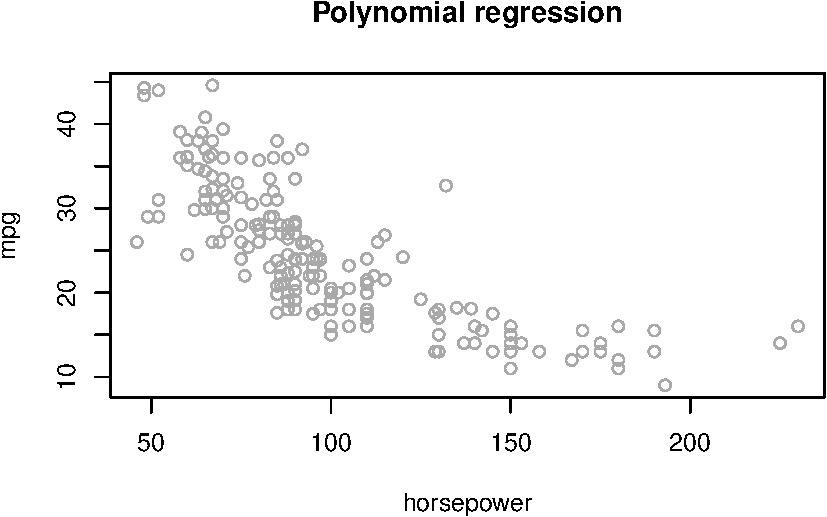
\includegraphics[width=0.5\linewidth]{RecEx9-sol_files/figure-latex/unnamed-chunk-1-1}

\begin{enumerate}
\def\labelenumi{\alph{enumi})}
\setcounter{enumi}{1}
\tightlist
\item
  Again, feel free to do this by hand. A simple R solution could look
  like this:
\end{enumerate}

\begin{Shaded}
\begin{Highlighting}[]
\KeywordTok{plot}\NormalTok{(}\OtherTok{NA}\NormalTok{,}\OtherTok{NA}\NormalTok{, }\CommentTok{# initialize a plot}
     \DataTypeTok{type =} \StringTok{"n"}\NormalTok{, }\CommentTok{# does not produce any points or lines}
     \DataTypeTok{xlim =} \KeywordTok{c}\NormalTok{(}\OperatorTok{-}\DecValTok{4}\NormalTok{,}\DecValTok{2}\NormalTok{),}\DataTypeTok{ylim =} \KeywordTok{c}\NormalTok{(}\OperatorTok{-}\DecValTok{1}\NormalTok{,}\DecValTok{5}\NormalTok{), }\DataTypeTok{xlab =} \KeywordTok{expression}\NormalTok{(X[}\DecValTok{1}\NormalTok{]), }\DataTypeTok{ylab =} \KeywordTok{expression}\NormalTok{(X[}\DecValTok{2}\NormalTok{]),}
     \DataTypeTok{asp =} \DecValTok{1}\NormalTok{)}
\KeywordTok{symbols}\NormalTok{(}\KeywordTok{c}\NormalTok{(}\OperatorTok{-}\DecValTok{1}\NormalTok{), }\KeywordTok{c}\NormalTok{(}\DecValTok{2}\NormalTok{), }\DataTypeTok{circles =} \KeywordTok{c}\NormalTok{(}\DecValTok{2}\NormalTok{), }\DataTypeTok{add =} \OtherTok{TRUE}\NormalTok{, }\DataTypeTok{inches =} \OtherTok{FALSE}\NormalTok{)}
\KeywordTok{text}\NormalTok{(}\KeywordTok{c}\NormalTok{(}\OperatorTok{-}\DecValTok{1}\NormalTok{), }\KeywordTok{c}\NormalTok{(}\DecValTok{2}\NormalTok{), }\StringTok{"< 4"}\NormalTok{)}
\KeywordTok{text}\NormalTok{(}\KeywordTok{c}\NormalTok{(}\OperatorTok{-}\DecValTok{4}\NormalTok{), }\KeywordTok{c}\NormalTok{(}\DecValTok{2}\NormalTok{), }\StringTok{"> 4"}\NormalTok{)}
\end{Highlighting}
\end{Shaded}

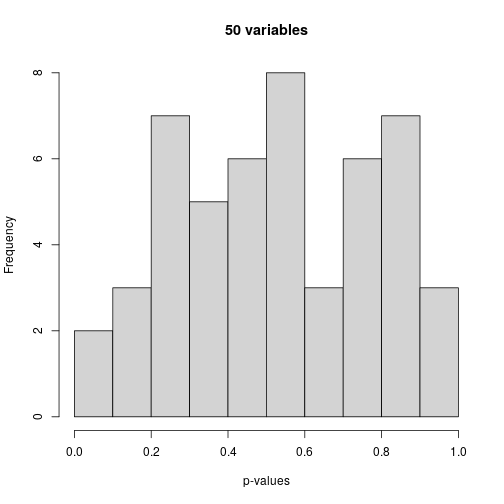
\includegraphics[width=0.5\linewidth]{RecEx9-sol_files/figure-latex/unnamed-chunk-2-1}

\begin{enumerate}
\def\labelenumi{\alph{enumi})}
\setcounter{enumi}{2}
\tightlist
\item
  You can do this by hand. Here we again use R and color the points
  according to the class they belong to:
\end{enumerate}

\begin{Shaded}
\begin{Highlighting}[]
\KeywordTok{plot}\NormalTok{(}\KeywordTok{c}\NormalTok{(}\DecValTok{0}\NormalTok{, }\DecValTok{-1}\NormalTok{, }\DecValTok{2}\NormalTok{, }\DecValTok{3}\NormalTok{), }\KeywordTok{c}\NormalTok{(}\DecValTok{0}\NormalTok{, }\DecValTok{1}\NormalTok{, }\DecValTok{2}\NormalTok{, }\DecValTok{8}\NormalTok{), }\DataTypeTok{col =} \KeywordTok{c}\NormalTok{(}\StringTok{"blue"}\NormalTok{, }\StringTok{"red"}\NormalTok{, }\StringTok{"blue"}\NormalTok{, }\StringTok{"blue"}\NormalTok{), }\DataTypeTok{type =} \StringTok{"p"}\NormalTok{, }
    \DataTypeTok{pch =} \DecValTok{19}\NormalTok{, }\DataTypeTok{asp =} \DecValTok{1}\NormalTok{, }\DataTypeTok{xlab =} \StringTok{"X1"}\NormalTok{, }\DataTypeTok{ylab =} \StringTok{"X2"}\NormalTok{)}
\KeywordTok{symbols}\NormalTok{(}\KeywordTok{c}\NormalTok{(}\OperatorTok{-}\DecValTok{1}\NormalTok{), }\KeywordTok{c}\NormalTok{(}\DecValTok{2}\NormalTok{), }\DataTypeTok{circles =} \KeywordTok{c}\NormalTok{(}\DecValTok{2}\NormalTok{), }\DataTypeTok{add =} \OtherTok{TRUE}\NormalTok{, }\DataTypeTok{inches =} \OtherTok{FALSE}\NormalTok{)}
\end{Highlighting}
\end{Shaded}

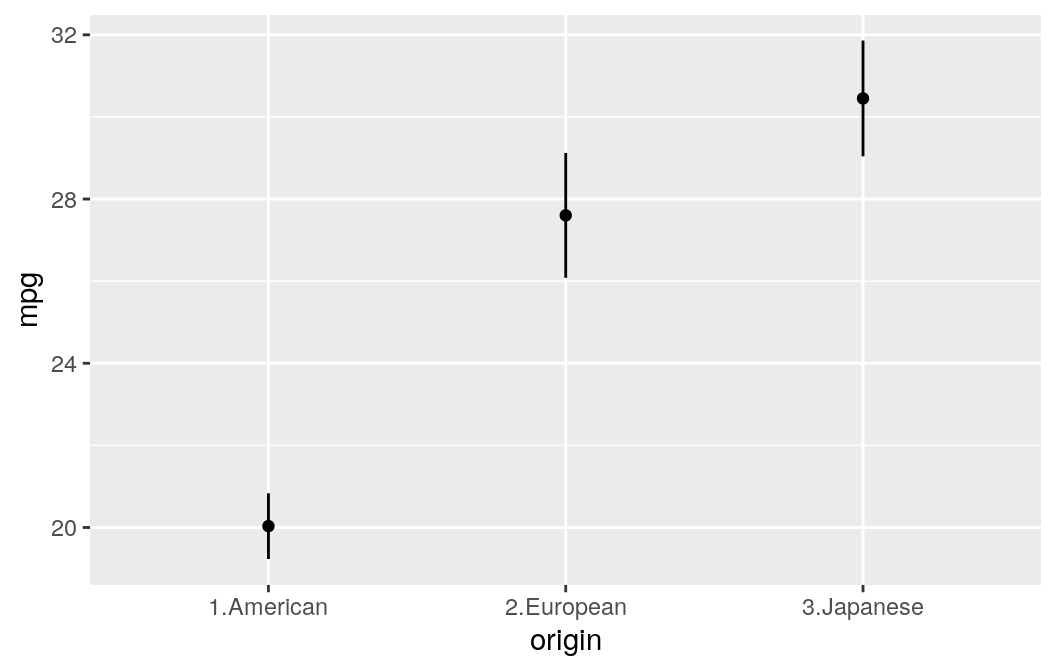
\includegraphics[width=0.5\linewidth]{RecEx9-sol_files/figure-latex/unnamed-chunk-3-1}

\begin{enumerate}
\def\labelenumi{\alph{enumi})}
\setcounter{enumi}{3}
\tightlist
\item
  Since equation \[(1 + X_1)^2 + (2 - X_2)^2 = 4.\] or
\end{enumerate}

\[ X_1^2 + X_2^2 + 2X_1 - 4X_2 +1 = 0\] includes quadratic terms, the
decision boundary is not linear, though it's linear in terms of
\(X_1^2,\) \(X_2^2,\) \(X_1,\) and \(X_2.\)

\hypertarget{problem-3}{%
\subsection{Problem 3}\label{problem-3}}

\begin{Shaded}
\begin{Highlighting}[]
\CommentTok{# code taken from video by Trevor Hastie}
\KeywordTok{set.seed}\NormalTok{(}\DecValTok{10111}\NormalTok{)}
\NormalTok{x <-}\StringTok{ }\KeywordTok{matrix}\NormalTok{(}\KeywordTok{rnorm}\NormalTok{(}\DecValTok{40}\NormalTok{), }\DecValTok{20}\NormalTok{, }\DecValTok{2}\NormalTok{)}
\NormalTok{y <-}\StringTok{ }\KeywordTok{rep}\NormalTok{(}\KeywordTok{c}\NormalTok{(}\OperatorTok{-}\DecValTok{1}\NormalTok{, }\DecValTok{1}\NormalTok{), }\KeywordTok{c}\NormalTok{(}\DecValTok{10}\NormalTok{, }\DecValTok{10}\NormalTok{))}
\NormalTok{x[y }\OperatorTok{==}\StringTok{ }\DecValTok{1}\NormalTok{, ] <-}\StringTok{ }\NormalTok{x[y }\OperatorTok{==}\StringTok{ }\DecValTok{1}\NormalTok{, ] }\OperatorTok{+}\StringTok{ }\DecValTok{1}
\KeywordTok{plot}\NormalTok{(x, }\DataTypeTok{col =}\NormalTok{ y }\OperatorTok{+}\StringTok{ }\DecValTok{3}\NormalTok{, }\DataTypeTok{pch =} \DecValTok{19}\NormalTok{, }\DataTypeTok{xlab =} \KeywordTok{expression}\NormalTok{(X[}\DecValTok{1}\NormalTok{]), }\DataTypeTok{ylab =} \KeywordTok{expression}\NormalTok{(X[}\DecValTok{2}\NormalTok{]))}
\end{Highlighting}
\end{Shaded}

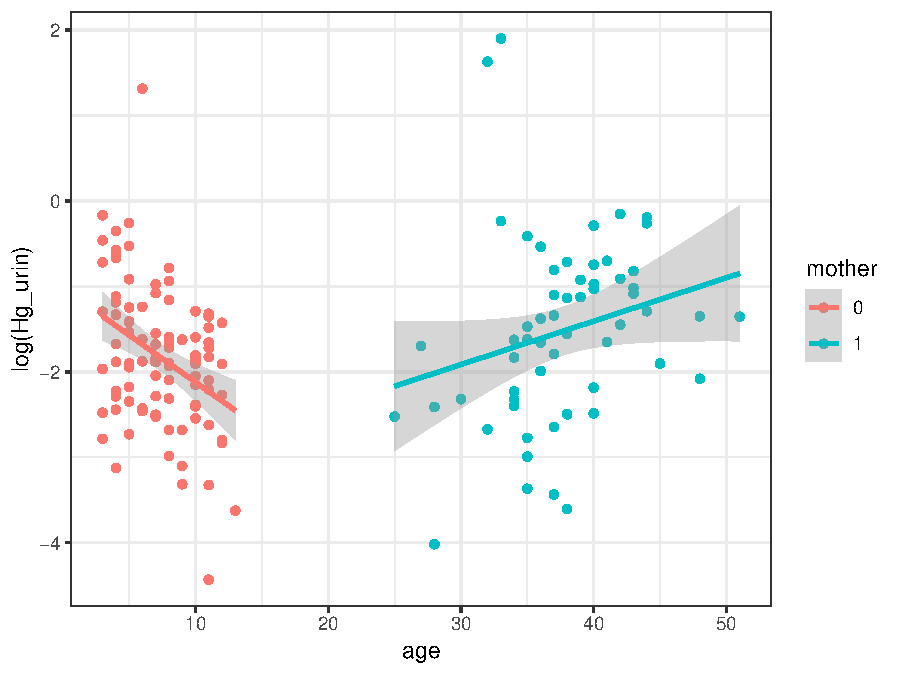
\includegraphics{RecEx9-sol_files/figure-latex/unnamed-chunk-4-1.pdf}

\begin{Shaded}
\begin{Highlighting}[]
\NormalTok{dat =}\StringTok{ }\KeywordTok{data.frame}\NormalTok{(x, }\DataTypeTok{y =} \KeywordTok{as.factor}\NormalTok{(y))}
\end{Highlighting}
\end{Shaded}

\begin{enumerate}
\def\labelenumi{(\alph{enumi})}
\item
\end{enumerate}

\begin{Shaded}
\begin{Highlighting}[]
\KeywordTok{library}\NormalTok{(e1071)}
\NormalTok{svmfit =}\StringTok{ }\KeywordTok{svm}\NormalTok{(y }\OperatorTok{~}\StringTok{ }\NormalTok{., }\DataTypeTok{data =}\NormalTok{ dat, }\DataTypeTok{kernel =} \StringTok{"linear"}\NormalTok{, }\DataTypeTok{cost =} \DecValTok{10}\NormalTok{, }\DataTypeTok{scale =} \OtherTok{FALSE}\NormalTok{)}

\CommentTok{# grid for plotting}
\NormalTok{make.grid =}\StringTok{ }\ControlFlowTok{function}\NormalTok{(x, }\DataTypeTok{n =} \DecValTok{75}\NormalTok{) \{}
    \CommentTok{# takes as input the data matrix x and number of grid points n in each direction}
    \CommentTok{# the default value will generate a 75x75 grid}
    
\NormalTok{    grange =}\StringTok{ }\KeywordTok{apply}\NormalTok{(x, }\DecValTok{2}\NormalTok{, range)  }\CommentTok{# range for x1 and x2}
\NormalTok{    x1 =}\StringTok{ }\KeywordTok{seq}\NormalTok{(}\DataTypeTok{from =}\NormalTok{ grange[}\DecValTok{1}\NormalTok{, }\DecValTok{1}\NormalTok{], }\DataTypeTok{to =}\NormalTok{ grange[}\DecValTok{2}\NormalTok{, }\DecValTok{1}\NormalTok{], }\DataTypeTok{length.out =}\NormalTok{ n)  }\CommentTok{# sequence from the lowest to the upper value of x1}
\NormalTok{    x2 =}\StringTok{ }\KeywordTok{seq}\NormalTok{(}\DataTypeTok{from =}\NormalTok{ grange[}\DecValTok{1}\NormalTok{, }\DecValTok{2}\NormalTok{], }\DataTypeTok{to =}\NormalTok{ grange[}\DecValTok{2}\NormalTok{, }\DecValTok{2}\NormalTok{], }\DataTypeTok{length.out =}\NormalTok{ n)  }\CommentTok{# sequence from the lowest to the upper value of x2}
    \KeywordTok{expand.grid}\NormalTok{(}\DataTypeTok{X1 =}\NormalTok{ x1, }\DataTypeTok{X2 =}\NormalTok{ x2)  }\CommentTok{#create a uniform grid according to x1 and x2 values}
\NormalTok{\}}
\end{Highlighting}
\end{Shaded}

\begin{Shaded}
\begin{Highlighting}[]
\NormalTok{x =}\StringTok{ }\KeywordTok{as.matrix}\NormalTok{(dat[, }\KeywordTok{c}\NormalTok{(}\StringTok{"X1"}\NormalTok{, }\StringTok{"X2"}\NormalTok{)])}
\NormalTok{xgrid =}\StringTok{ }\KeywordTok{make.grid}\NormalTok{(x)}
\NormalTok{ygrid =}\StringTok{ }\KeywordTok{predict}\NormalTok{(svmfit, xgrid)}
\KeywordTok{plot}\NormalTok{(xgrid, }\DataTypeTok{col =} \KeywordTok{c}\NormalTok{(}\StringTok{"red"}\NormalTok{, }\StringTok{"blue"}\NormalTok{)[}\KeywordTok{as.numeric}\NormalTok{(ygrid)], }\DataTypeTok{pch =} \DecValTok{20}\NormalTok{, }\DataTypeTok{cex =} \FloatTok{0.2}\NormalTok{)}
\end{Highlighting}
\end{Shaded}

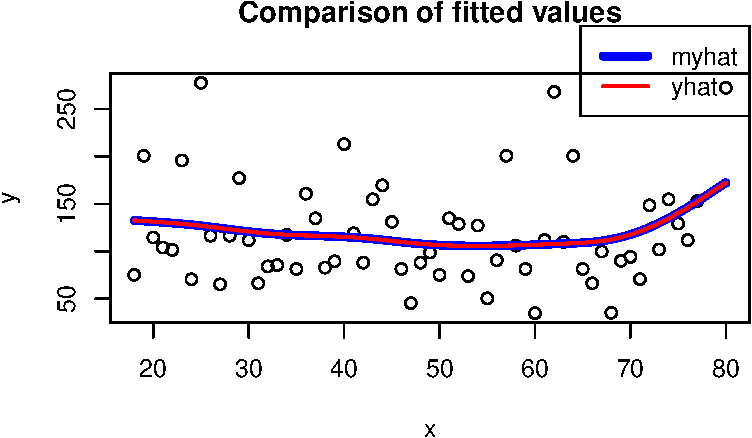
\includegraphics{RecEx9-sol_files/figure-latex/unnamed-chunk-6-1.pdf}

\begin{enumerate}
\def\labelenumi{(\alph{enumi})}
\setcounter{enumi}{1}
\item
\end{enumerate}

\begin{Shaded}
\begin{Highlighting}[]
\KeywordTok{plot}\NormalTok{(xgrid, }\DataTypeTok{col =} \KeywordTok{c}\NormalTok{(}\StringTok{"red"}\NormalTok{, }\StringTok{"blue"}\NormalTok{)[}\KeywordTok{as.numeric}\NormalTok{(ygrid)], }\DataTypeTok{pch =} \DecValTok{20}\NormalTok{, }\DataTypeTok{cex =} \FloatTok{0.2}\NormalTok{)}
\KeywordTok{points}\NormalTok{(x, }\DataTypeTok{col =}\NormalTok{ y }\OperatorTok{+}\StringTok{ }\DecValTok{3}\NormalTok{, }\DataTypeTok{pch =} \DecValTok{19}\NormalTok{)}
\KeywordTok{points}\NormalTok{(x[svmfit}\OperatorTok{$}\NormalTok{index, ], }\DataTypeTok{pch =} \DecValTok{5}\NormalTok{, }\DataTypeTok{cex =} \DecValTok{2}\NormalTok{)}
\end{Highlighting}
\end{Shaded}

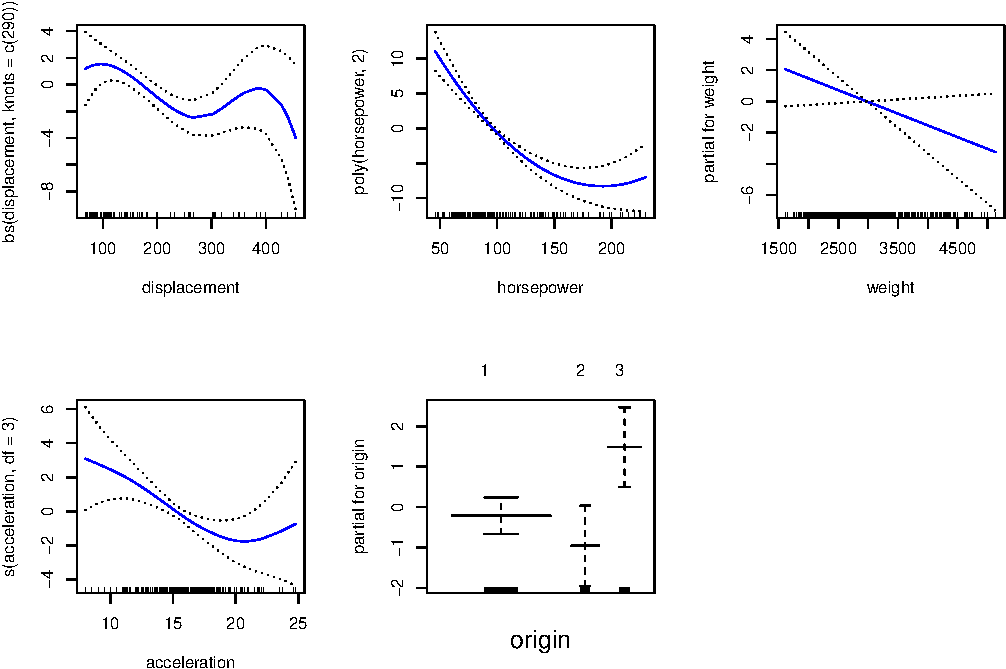
\includegraphics{RecEx9-sol_files/figure-latex/unnamed-chunk-7-1.pdf}

\begin{enumerate}
\def\labelenumi{(\alph{enumi})}
\setcounter{enumi}{2}
\item
\end{enumerate}

\begin{Shaded}
\begin{Highlighting}[]
\NormalTok{beta =}\StringTok{ }\KeywordTok{drop}\NormalTok{(}\KeywordTok{t}\NormalTok{(svmfit}\OperatorTok{$}\NormalTok{coefs) }\OperatorTok\StringTok{ }\NormalTok{x[svmfit}\OperatorTok{$}\NormalTok{index, ])}
\NormalTok{beta0 =}\StringTok{ }\NormalTok{svmfit}\OperatorTok{$}\NormalTok{rho}
\KeywordTok{plot}\NormalTok{(xgrid, }\DataTypeTok{col =} \KeywordTok{c}\NormalTok{(}\StringTok{"red"}\NormalTok{, }\StringTok{"blue"}\NormalTok{)[}\KeywordTok{as.numeric}\NormalTok{(ygrid)], }\DataTypeTok{pch =} \DecValTok{20}\NormalTok{, }\DataTypeTok{cex =} \FloatTok{0.2}\NormalTok{)}
\KeywordTok{points}\NormalTok{(x, }\DataTypeTok{col =}\NormalTok{ y }\OperatorTok{+}\StringTok{ }\DecValTok{3}\NormalTok{, }\DataTypeTok{pch =} \DecValTok{19}\NormalTok{)}
\KeywordTok{points}\NormalTok{(x[svmfit}\OperatorTok{$}\NormalTok{index, ], }\DataTypeTok{pch =} \DecValTok{5}\NormalTok{, }\DataTypeTok{cex =} \DecValTok{2}\NormalTok{)}
\KeywordTok{abline}\NormalTok{(beta0}\OperatorTok{/}\NormalTok{beta[}\DecValTok{2}\NormalTok{], }\OperatorTok{-}\NormalTok{beta[}\DecValTok{1}\NormalTok{]}\OperatorTok{/}\NormalTok{beta[}\DecValTok{2}\NormalTok{], }\DataTypeTok{lwd =} \DecValTok{2}\NormalTok{)  }\CommentTok{#class boundary}
\KeywordTok{abline}\NormalTok{((beta0 }\OperatorTok{-}\StringTok{ }\DecValTok{1}\NormalTok{)}\OperatorTok{/}\NormalTok{beta[}\DecValTok{2}\NormalTok{], }\OperatorTok{-}\NormalTok{beta[}\DecValTok{1}\NormalTok{]}\OperatorTok{/}\NormalTok{beta[}\DecValTok{2}\NormalTok{], }\DataTypeTok{lty =} \DecValTok{2}\NormalTok{)  }\CommentTok{#class boundary-margin}
\KeywordTok{abline}\NormalTok{((beta0 }\OperatorTok{+}\StringTok{ }\DecValTok{1}\NormalTok{)}\OperatorTok{/}\NormalTok{beta[}\DecValTok{2}\NormalTok{], }\OperatorTok{-}\NormalTok{beta[}\DecValTok{1}\NormalTok{]}\OperatorTok{/}\NormalTok{beta[}\DecValTok{2}\NormalTok{], }\DataTypeTok{lty =} \DecValTok{2}\NormalTok{)  }\CommentTok{#class boundary+margin}
\end{Highlighting}
\end{Shaded}

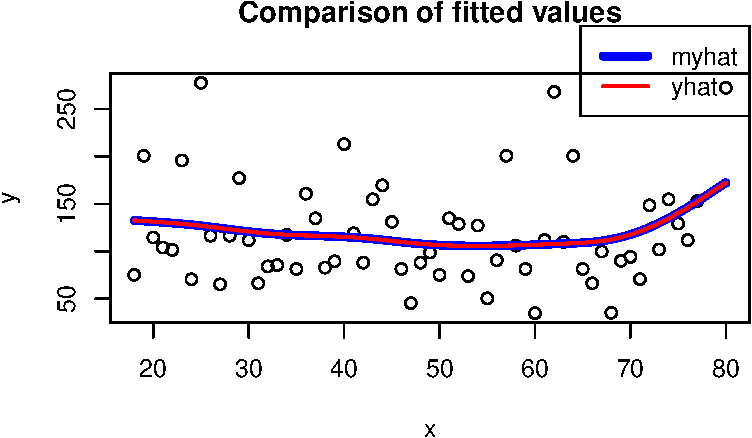
\includegraphics{RecEx9-sol_files/figure-latex/unnamed-chunk-8-1.pdf}

\hypertarget{problem-4}{%
\subsection{Problem 4}\label{problem-4}}

\begin{Shaded}
\begin{Highlighting}[]
\KeywordTok{load}\NormalTok{(}\KeywordTok{url}\NormalTok{(}\StringTok{"https://web.stanford.edu/~hastie/ElemStatLearn/datasets/ESL.mixture.rda"}\NormalTok{))}
\CommentTok{# names(ESL.mixture)}
\KeywordTok{rm}\NormalTok{(x, y)}
\KeywordTok{attach}\NormalTok{(ESL.mixture)}
\KeywordTok{plot}\NormalTok{(x, }\DataTypeTok{col =}\NormalTok{ y }\OperatorTok{+}\StringTok{ }\DecValTok{1}\NormalTok{, }\DataTypeTok{pch =} \DecValTok{19}\NormalTok{, }\DataTypeTok{xlab =} \KeywordTok{expression}\NormalTok{(X[}\DecValTok{1}\NormalTok{]), }\DataTypeTok{ylab =} \KeywordTok{expression}\NormalTok{(X[}\DecValTok{2}\NormalTok{]))}
\end{Highlighting}
\end{Shaded}

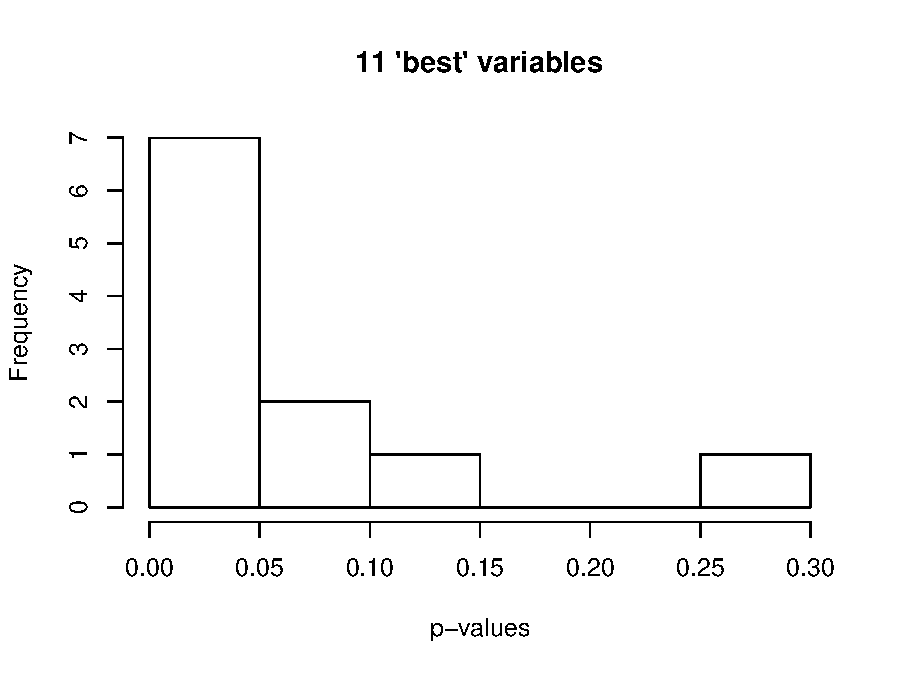
\includegraphics[width=0.55\linewidth]{RecEx9-sol_files/figure-latex/unnamed-chunk-9-1}

\begin{Shaded}
\begin{Highlighting}[]
\NormalTok{dat =}\StringTok{ }\KeywordTok{data.frame}\NormalTok{(}\DataTypeTok{y =} \KeywordTok{factor}\NormalTok{(y), x)}
\end{Highlighting}
\end{Shaded}

\begin{Shaded}
\begin{Highlighting}[]
\NormalTok{r.cv <-}\StringTok{ }\KeywordTok{tune}\NormalTok{(svm, }\KeywordTok{factor}\NormalTok{(y) }\OperatorTok{~}\StringTok{ }\NormalTok{., }\DataTypeTok{data =}\NormalTok{ dat, }\DataTypeTok{kernel =} \StringTok{"radial"}\NormalTok{, }\DataTypeTok{ranges =} \KeywordTok{list}\NormalTok{(}\DataTypeTok{cost =} \KeywordTok{c}\NormalTok{(}\FloatTok{0.01}\NormalTok{, }
    \FloatTok{0.1}\NormalTok{, }\DecValTok{1}\NormalTok{, }\DecValTok{5}\NormalTok{, }\DecValTok{10}\NormalTok{, }\DecValTok{100}\NormalTok{, }\DecValTok{1000}\NormalTok{), }\DataTypeTok{gamma =} \KeywordTok{c}\NormalTok{(}\FloatTok{0.01}\NormalTok{, }\FloatTok{0.1}\NormalTok{, }\DecValTok{1}\NormalTok{, }\DecValTok{10}\NormalTok{, }\DecValTok{100}\NormalTok{)))}
\KeywordTok{summary}\NormalTok{(r.cv)}
\end{Highlighting}
\end{Shaded}

\begin{verbatim}
## 
## Parameter tuning of 'svm':
## 
## - sampling method: 10-fold cross validation 
## 
## - best parameters:
##  cost gamma
##     1    10
## 
## - best performance: 0.165 
## 
## - Detailed performance results:
##     cost gamma error dispersion
## 1  1e-02 1e-02 0.525 0.14191155
## 2  1e-01 1e-02 0.525 0.14191155
## 3  1e+00 1e-02 0.285 0.08834906
## 4  5e+00 1e-02 0.320 0.06749486
## 5  1e+01 1e-02 0.315 0.07472171
## 6  1e+02 1e-02 0.310 0.07745967
## 7  1e+03 1e-02 0.295 0.07245688
## 8  1e-02 1e-01 0.525 0.14191155
## 9  1e-01 1e-01 0.305 0.07975657
## 10 1e+00 1e-01 0.325 0.07546154
## 11 5e+00 1e-01 0.295 0.07245688
## 12 1e+01 1e-01 0.290 0.06992059
## 13 1e+02 1e-01 0.290 0.06146363
## 14 1e+03 1e-01 0.215 0.04743416
## 15 1e-02 1e+00 0.535 0.12258784
## 16 1e-01 1e+00 0.285 0.06258328
## 17 1e+00 1e+00 0.205 0.04377975
## 18 5e+00 1e+00 0.175 0.03535534
## 19 1e+01 1e+00 0.180 0.04830459
## 20 1e+02 1e+00 0.185 0.05797509
## 21 1e+03 1e+00 0.190 0.07378648
## 22 1e-02 1e+01 0.495 0.19923465
## 23 1e-01 1e+01 0.465 0.18715709
## 24 1e+00 1e+01 0.165 0.07472171
## 25 5e+00 1e+01 0.195 0.06851602
## 26 1e+01 1e+01 0.215 0.06258328
## 27 1e+02 1e+01 0.270 0.10327956
## 28 1e+03 1e+01 0.300 0.10540926
## 29 1e-02 1e+02 0.505 0.18173546
## 30 1e-01 1e+02 0.505 0.18173546
## 31 1e+00 1e+02 0.315 0.15284342
## 32 5e+00 1e+02 0.305 0.12122064
## 33 1e+01 1e+02 0.315 0.12258784
## 34 1e+02 1e+02 0.310 0.12202003
## 35 1e+03 1e+02 0.310 0.12202003
\end{verbatim}

\begin{Shaded}
\begin{Highlighting}[]
\NormalTok{fit <-}\StringTok{ }\NormalTok{r.cv}\OperatorTok{$}\NormalTok{best.model}
\end{Highlighting}
\end{Shaded}

Now we plot the non-linear decision boundary, and add the training
points.

\begin{Shaded}
\begin{Highlighting}[]
\NormalTok{xgrid =}\StringTok{ }\KeywordTok{make.grid}\NormalTok{(x)}
\NormalTok{ygrid =}\StringTok{ }\KeywordTok{predict}\NormalTok{(fit, xgrid)}
\KeywordTok{plot}\NormalTok{(xgrid, }\DataTypeTok{col =} \KeywordTok{as.numeric}\NormalTok{(ygrid), }\DataTypeTok{pch =} \DecValTok{20}\NormalTok{, }\DataTypeTok{cex =} \FloatTok{0.2}\NormalTok{)}
\KeywordTok{points}\NormalTok{(x, }\DataTypeTok{col =}\NormalTok{ y }\OperatorTok{+}\StringTok{ }\DecValTok{1}\NormalTok{, }\DataTypeTok{pch =} \DecValTok{19}\NormalTok{)}

\CommentTok{# decision boundary}
\NormalTok{func =}\StringTok{ }\KeywordTok{predict}\NormalTok{(fit, xgrid, }\DataTypeTok{decision.values =} \OtherTok{TRUE}\NormalTok{)}
\NormalTok{func =}\StringTok{ }\KeywordTok{attributes}\NormalTok{(func)}\OperatorTok{$}\NormalTok{decision}
\KeywordTok{contour}\NormalTok{(}\KeywordTok{unique}\NormalTok{(xgrid[, }\DecValTok{1}\NormalTok{]), }\KeywordTok{unique}\NormalTok{(xgrid[, }\DecValTok{2}\NormalTok{]), }\KeywordTok{matrix}\NormalTok{(func, }\DecValTok{75}\NormalTok{, }\DecValTok{75}\NormalTok{), }\DataTypeTok{level =} \DecValTok{0}\NormalTok{, }
    \DataTypeTok{add =} \OtherTok{TRUE}\NormalTok{)  }\CommentTok{#svm boundary}
\end{Highlighting}
\end{Shaded}

\includegraphics{RecEx9-sol_files/figure-latex/unnamed-chunk-11-1.pdf}

\hypertarget{problem-5}{%
\subsection{Problem 5}\label{problem-5}}

\begin{enumerate}
\def\labelenumi{(\alph{enumi})}
\item
\end{enumerate}

\begin{Shaded}
\begin{Highlighting}[]
\KeywordTok{library}\NormalTok{(ISLR)}
\KeywordTok{data}\NormalTok{(OJ)}
\CommentTok{# head(OJ)}
\NormalTok{n =}\StringTok{ }\KeywordTok{nrow}\NormalTok{(OJ)}
\KeywordTok{set.seed}\NormalTok{(}\DecValTok{4268}\NormalTok{)}
\NormalTok{train =}\StringTok{ }\KeywordTok{sample}\NormalTok{(}\DecValTok{1}\OperatorTok{:}\NormalTok{n, }\DecValTok{800}\NormalTok{)}
\NormalTok{OJ.train =}\StringTok{ }\NormalTok{OJ[train, ]}
\NormalTok{OJ.test =}\StringTok{ }\NormalTok{OJ[}\OperatorTok{-}\NormalTok{train, ]}
\end{Highlighting}
\end{Shaded}

\begin{enumerate}
\def\labelenumi{(\alph{enumi})}
\setcounter{enumi}{1}
\item
\end{enumerate}

\begin{Shaded}
\begin{Highlighting}[]
\KeywordTok{library}\NormalTok{(e1071)}
\NormalTok{linear =}\StringTok{ }\KeywordTok{svm}\NormalTok{(Purchase }\OperatorTok{~}\StringTok{ }\NormalTok{., }\DataTypeTok{data =}\NormalTok{ OJ, }\DataTypeTok{subset =}\NormalTok{ train, }\DataTypeTok{kernel =} \StringTok{"linear"}\NormalTok{, }\DataTypeTok{cost =} \FloatTok{0.01}\NormalTok{)}
\KeywordTok{summary}\NormalTok{(linear)}
\end{Highlighting}
\end{Shaded}

\begin{verbatim}
## 
## Call:
## svm(formula = Purchase ~ ., data = OJ, kernel = "linear", cost = 0.01, 
##     subset = train)
## 
## 
## Parameters:
##    SVM-Type:  C-classification 
##  SVM-Kernel:  linear 
##        cost:  0.01 
## 
## Number of Support Vectors:  431
## 
##  ( 217 214 )
## 
## 
## Number of Classes:  2 
## 
## Levels: 
##  CH MM
\end{verbatim}

We have 431 Support vectors, where 217 belong to the class CH (Citrus
Hill) and 214 belong to the class MM (Minute Maid Orange Juice).

\begin{enumerate}
\def\labelenumi{(\alph{enumi})}
\setcounter{enumi}{2}
\item
\end{enumerate}

\begin{Shaded}
\begin{Highlighting}[]
\NormalTok{pred.train =}\StringTok{ }\KeywordTok{predict}\NormalTok{(linear, OJ.train)}
\NormalTok{(}\DataTypeTok{ta =} \KeywordTok{table}\NormalTok{(OJ.train}\OperatorTok{$}\NormalTok{Purchase, pred.train))}
\end{Highlighting}
\end{Shaded}

\begin{verbatim}
##     pred.train
##       CH  MM
##   CH 431  56
##   MM  78 235
\end{verbatim}

\begin{Shaded}
\begin{Highlighting}[]
\NormalTok{msrate =}\StringTok{ }\DecValTok{1} \OperatorTok{-}\StringTok{ }\KeywordTok{sum}\NormalTok{(}\KeywordTok{diag}\NormalTok{(ta))}\OperatorTok{/}\KeywordTok{sum}\NormalTok{(ta)}
\NormalTok{msrate}
\end{Highlighting}
\end{Shaded}

\begin{verbatim}
## [1] 0.1675
\end{verbatim}

\begin{Shaded}
\begin{Highlighting}[]
\NormalTok{pred.test =}\StringTok{ }\KeywordTok{predict}\NormalTok{(linear, OJ.test)}
\NormalTok{(}\DataTypeTok{ta =} \KeywordTok{table}\NormalTok{(OJ.test}\OperatorTok{$}\NormalTok{Purchase, pred.test))}
\end{Highlighting}
\end{Shaded}

\begin{verbatim}
##     pred.test
##       CH  MM
##   CH 143  23
##   MM  25  79
\end{verbatim}

\begin{Shaded}
\begin{Highlighting}[]
\NormalTok{msrate =}\StringTok{ }\DecValTok{1} \OperatorTok{-}\StringTok{ }\KeywordTok{sum}\NormalTok{(}\KeywordTok{diag}\NormalTok{(ta))}\OperatorTok{/}\KeywordTok{sum}\NormalTok{(ta)}
\NormalTok{msrate}
\end{Highlighting}
\end{Shaded}

\begin{verbatim}
## [1] 0.1777778
\end{verbatim}

\begin{enumerate}
\def\labelenumi{(\alph{enumi})}
\setcounter{enumi}{3}
\item
\end{enumerate}

\begin{Shaded}
\begin{Highlighting}[]
\KeywordTok{set.seed}\NormalTok{(}\DecValTok{4268}\NormalTok{)}
\NormalTok{cost.val =}\StringTok{ }\DecValTok{10}\OperatorTok{^}\KeywordTok{seq}\NormalTok{(}\OperatorTok{-}\DecValTok{2}\NormalTok{, }\DecValTok{1}\NormalTok{, }\DataTypeTok{by =} \FloatTok{0.25}\NormalTok{)}
\NormalTok{tune.cost =}\StringTok{ }\KeywordTok{tune}\NormalTok{(svm, Purchase }\OperatorTok{~}\StringTok{ }\NormalTok{., }\DataTypeTok{data =}\NormalTok{ OJ.train, }\DataTypeTok{kernel =} \StringTok{"linear"}\NormalTok{, }\DataTypeTok{ranges =} \KeywordTok{list}\NormalTok{(}\DataTypeTok{cost =}\NormalTok{ cost.val))}
\CommentTok{# summary(tune.cost)}
\end{Highlighting}
\end{Shaded}

\begin{enumerate}
\def\labelenumi{(\alph{enumi})}
\setcounter{enumi}{4}
\item
\end{enumerate}

\begin{Shaded}
\begin{Highlighting}[]
\NormalTok{svm.linear =}\StringTok{ }\KeywordTok{svm}\NormalTok{(Purchase }\OperatorTok{~}\StringTok{ }\NormalTok{., }\DataTypeTok{kernel =} \StringTok{"linear"}\NormalTok{, }\DataTypeTok{data =}\NormalTok{ OJ.train, }\DataTypeTok{cost =}\NormalTok{ tune.cost}\OperatorTok{$}\NormalTok{best.parameter}\OperatorTok{$}\NormalTok{cost)}
\NormalTok{train.pred =}\StringTok{ }\KeywordTok{predict}\NormalTok{(svm.linear, OJ.train)}
\end{Highlighting}
\end{Shaded}

\begin{Shaded}
\begin{Highlighting}[]
\NormalTok{(}\DataTypeTok{ta =} \KeywordTok{table}\NormalTok{(OJ.train}\OperatorTok{$}\NormalTok{Purchase, train.pred))}
\end{Highlighting}
\end{Shaded}

\begin{verbatim}
##     train.pred
##       CH  MM
##   CH 434  53
##   MM  73 240
\end{verbatim}

\begin{Shaded}
\begin{Highlighting}[]
\NormalTok{msrate.train.linear =}\StringTok{ }\DecValTok{1} \OperatorTok{-}\StringTok{ }\KeywordTok{sum}\NormalTok{(}\KeywordTok{diag}\NormalTok{(ta))}\OperatorTok{/}\KeywordTok{sum}\NormalTok{(ta)}
\NormalTok{msrate.train.linear}
\end{Highlighting}
\end{Shaded}

\begin{verbatim}
## [1] 0.1575
\end{verbatim}

\begin{Shaded}
\begin{Highlighting}[]
\NormalTok{test.pred =}\StringTok{ }\KeywordTok{predict}\NormalTok{(svm.linear, OJ.test)}
\NormalTok{(}\DataTypeTok{ta =} \KeywordTok{table}\NormalTok{(OJ.test}\OperatorTok{$}\NormalTok{Purchase, test.pred))}
\end{Highlighting}
\end{Shaded}

\begin{verbatim}
##     test.pred
##       CH  MM
##   CH 143  23
##   MM  23  81
\end{verbatim}

\begin{Shaded}
\begin{Highlighting}[]
\NormalTok{msrate.test.linear =}\StringTok{ }\DecValTok{1} \OperatorTok{-}\StringTok{ }\KeywordTok{sum}\NormalTok{(}\KeywordTok{diag}\NormalTok{(ta))}\OperatorTok{/}\KeywordTok{sum}\NormalTok{(ta)}
\NormalTok{msrate.test.linear}
\end{Highlighting}
\end{Shaded}

\begin{verbatim}
## [1] 0.1703704
\end{verbatim}

\begin{enumerate}
\def\labelenumi{(\alph{enumi})}
\setcounter{enumi}{5}
\tightlist
\item
  Radial Kernel Model
\end{enumerate}

\begin{Shaded}
\begin{Highlighting}[]
\NormalTok{svm.radial =}\StringTok{ }\KeywordTok{svm}\NormalTok{(Purchase }\OperatorTok{~}\StringTok{ }\NormalTok{., }\DataTypeTok{kernel =} \StringTok{"radial"}\NormalTok{, }\DataTypeTok{data =}\NormalTok{ OJ.train)}
\CommentTok{# summary(svm.radial)}
\end{Highlighting}
\end{Shaded}

Train and test error rate

\begin{Shaded}
\begin{Highlighting}[]
\NormalTok{pred.train =}\StringTok{ }\KeywordTok{predict}\NormalTok{(svm.radial, OJ.train)}
\NormalTok{(}\DataTypeTok{ta =} \KeywordTok{table}\NormalTok{(OJ.train}\OperatorTok{$}\NormalTok{Purchase, pred.train))}
\end{Highlighting}
\end{Shaded}

\begin{verbatim}
##     pred.train
##       CH  MM
##   CH 446  41
##   MM  72 241
\end{verbatim}

\begin{Shaded}
\begin{Highlighting}[]
\NormalTok{msrate.train.radial =}\StringTok{ }\DecValTok{1} \OperatorTok{-}\StringTok{ }\KeywordTok{sum}\NormalTok{(}\KeywordTok{diag}\NormalTok{(ta))}\OperatorTok{/}\KeywordTok{sum}\NormalTok{(ta)}
\NormalTok{msrate.train.radial}
\end{Highlighting}
\end{Shaded}

\begin{verbatim}
## [1] 0.14125
\end{verbatim}

\begin{Shaded}
\begin{Highlighting}[]
\NormalTok{pred.test =}\StringTok{ }\KeywordTok{predict}\NormalTok{(svm.radial, OJ.test)}
\NormalTok{(}\DataTypeTok{ta =} \KeywordTok{table}\NormalTok{(OJ.test}\OperatorTok{$}\NormalTok{Purchase, pred.test))}
\end{Highlighting}
\end{Shaded}

\begin{verbatim}
##     pred.test
##       CH  MM
##   CH 145  21
##   MM  25  79
\end{verbatim}

\begin{Shaded}
\begin{Highlighting}[]
\NormalTok{msrate.test.radial =}\StringTok{ }\DecValTok{1} \OperatorTok{-}\StringTok{ }\KeywordTok{sum}\NormalTok{(}\KeywordTok{diag}\NormalTok{(ta))}\OperatorTok{/}\KeywordTok{sum}\NormalTok{(ta)}
\NormalTok{msrate.test.radial}
\end{Highlighting}
\end{Shaded}

\begin{verbatim}
## [1] 0.1703704
\end{verbatim}

Optimal cost

\begin{Shaded}
\begin{Highlighting}[]
\KeywordTok{set.seed}\NormalTok{(}\DecValTok{4268}\NormalTok{)}
\NormalTok{cost.val =}\StringTok{ }\DecValTok{10}\OperatorTok{^}\KeywordTok{seq}\NormalTok{(}\OperatorTok{-}\DecValTok{2}\NormalTok{, }\DecValTok{1}\NormalTok{, }\DataTypeTok{by =} \FloatTok{0.25}\NormalTok{)}
\NormalTok{tune.cost =}\StringTok{ }\KeywordTok{tune}\NormalTok{(svm, Purchase }\OperatorTok{~}\StringTok{ }\NormalTok{., }\DataTypeTok{data =}\NormalTok{ OJ.train, }\DataTypeTok{kernel =} \StringTok{"radial"}\NormalTok{, }\DataTypeTok{ranges =} \KeywordTok{list}\NormalTok{(}\DataTypeTok{cost =}\NormalTok{ cost.val))}
\CommentTok{# summary(tune.cost)}
\end{Highlighting}
\end{Shaded}

\begin{Shaded}
\begin{Highlighting}[]
\NormalTok{svm.radial =}\StringTok{ }\KeywordTok{svm}\NormalTok{(Purchase }\OperatorTok{~}\StringTok{ }\NormalTok{., }\DataTypeTok{kernel =} \StringTok{"radial"}\NormalTok{, }\DataTypeTok{data =}\NormalTok{ OJ.train, }\DataTypeTok{cost =}\NormalTok{ tune.cost}\OperatorTok{$}\NormalTok{best.parameter}\OperatorTok{$}\NormalTok{cost)}
\NormalTok{train.pred =}\StringTok{ }\KeywordTok{predict}\NormalTok{(svm.radial, OJ.train)}
\end{Highlighting}
\end{Shaded}

Train and test error for optimal cost

\begin{Shaded}
\begin{Highlighting}[]
\NormalTok{(}\DataTypeTok{ta =} \KeywordTok{table}\NormalTok{(OJ.train}\OperatorTok{$}\NormalTok{Purchase, train.pred))}
\end{Highlighting}
\end{Shaded}

\begin{verbatim}
##     train.pred
##       CH  MM
##   CH 450  37
##   MM  73 240
\end{verbatim}

\begin{Shaded}
\begin{Highlighting}[]
\NormalTok{msrate.train.linear =}\StringTok{ }\DecValTok{1} \OperatorTok{-}\StringTok{ }\KeywordTok{sum}\NormalTok{(}\KeywordTok{diag}\NormalTok{(ta))}\OperatorTok{/}\KeywordTok{sum}\NormalTok{(ta)}
\NormalTok{msrate.train.linear}
\end{Highlighting}
\end{Shaded}

\begin{verbatim}
## [1] 0.1375
\end{verbatim}

\begin{Shaded}
\begin{Highlighting}[]
\NormalTok{test.pred =}\StringTok{ }\KeywordTok{predict}\NormalTok{(svm.radial, OJ.test)}
\NormalTok{(}\DataTypeTok{ta =} \KeywordTok{table}\NormalTok{(OJ.test}\OperatorTok{$}\NormalTok{Purchase, test.pred))}
\end{Highlighting}
\end{Shaded}

\begin{verbatim}
##     test.pred
##       CH  MM
##   CH 146  20
##   MM  28  76
\end{verbatim}

\begin{Shaded}
\begin{Highlighting}[]
\NormalTok{msrate.test.linear =}\StringTok{ }\DecValTok{1} \OperatorTok{-}\StringTok{ }\KeywordTok{sum}\NormalTok{(}\KeywordTok{diag}\NormalTok{(ta))}\OperatorTok{/}\KeywordTok{sum}\NormalTok{(ta)}
\NormalTok{msrate.test.linear}
\end{Highlighting}
\end{Shaded}

\begin{verbatim}
## [1] 0.1777778
\end{verbatim}

\begin{enumerate}
\def\labelenumi{(\alph{enumi})}
\setcounter{enumi}{6}
\tightlist
\item
  Polynomial Kernel Model of degree 2
\end{enumerate}

\begin{Shaded}
\begin{Highlighting}[]
\NormalTok{svm.poly =}\StringTok{ }\KeywordTok{svm}\NormalTok{(Purchase }\OperatorTok{~}\StringTok{ }\NormalTok{., }\DataTypeTok{kernel =} \StringTok{"polynomial"}\NormalTok{, }\DataTypeTok{degree =} \DecValTok{2}\NormalTok{, }\DataTypeTok{data =}\NormalTok{ OJ.train)}
\CommentTok{# summary(svm.poly)}
\end{Highlighting}
\end{Shaded}

Train and test error rate

\begin{Shaded}
\begin{Highlighting}[]
\NormalTok{pred.train =}\StringTok{ }\KeywordTok{predict}\NormalTok{(svm.poly, OJ.train)}
\NormalTok{(}\DataTypeTok{ta =} \KeywordTok{table}\NormalTok{(OJ.train}\OperatorTok{$}\NormalTok{Purchase, pred.train))}
\end{Highlighting}
\end{Shaded}

\begin{verbatim}
##     pred.train
##       CH  MM
##   CH 453  34
##   MM 109 204
\end{verbatim}

\begin{Shaded}
\begin{Highlighting}[]
\NormalTok{msrate.train.poly =}\StringTok{ }\DecValTok{1} \OperatorTok{-}\StringTok{ }\KeywordTok{sum}\NormalTok{(}\KeywordTok{diag}\NormalTok{(ta))}\OperatorTok{/}\KeywordTok{sum}\NormalTok{(ta)}
\NormalTok{msrate.train.poly}
\end{Highlighting}
\end{Shaded}

\begin{verbatim}
## [1] 0.17875
\end{verbatim}

\begin{Shaded}
\begin{Highlighting}[]
\NormalTok{pred.test =}\StringTok{ }\KeywordTok{predict}\NormalTok{(svm.poly, OJ.test)}
\NormalTok{(}\DataTypeTok{ta =} \KeywordTok{table}\NormalTok{(OJ.test}\OperatorTok{$}\NormalTok{Purchase, pred.test))}
\end{Highlighting}
\end{Shaded}

\begin{verbatim}
##     pred.test
##       CH  MM
##   CH 152  14
##   MM  33  71
\end{verbatim}

\begin{Shaded}
\begin{Highlighting}[]
\NormalTok{msrate.test.poly =}\StringTok{ }\DecValTok{1} \OperatorTok{-}\StringTok{ }\KeywordTok{sum}\NormalTok{(}\KeywordTok{diag}\NormalTok{(ta))}\OperatorTok{/}\KeywordTok{sum}\NormalTok{(ta)}
\NormalTok{msrate.test.poly}
\end{Highlighting}
\end{Shaded}

\begin{verbatim}
## [1] 0.1740741
\end{verbatim}

Optimal cost

\begin{Shaded}
\begin{Highlighting}[]
\KeywordTok{set.seed}\NormalTok{(}\DecValTok{4268}\NormalTok{)}
\NormalTok{cost.val =}\StringTok{ }\DecValTok{10}\OperatorTok{^}\KeywordTok{seq}\NormalTok{(}\OperatorTok{-}\DecValTok{2}\NormalTok{, }\DecValTok{1}\NormalTok{, }\DataTypeTok{by =} \FloatTok{0.25}\NormalTok{)}
\NormalTok{tune.cost =}\StringTok{ }\KeywordTok{tune}\NormalTok{(svm, Purchase }\OperatorTok{~}\StringTok{ }\NormalTok{., }\DataTypeTok{data =}\NormalTok{ OJ.train, }\DataTypeTok{kernel =} \StringTok{"poly"}\NormalTok{, }\DataTypeTok{degree =} \DecValTok{2}\NormalTok{, }
    \DataTypeTok{ranges =} \KeywordTok{list}\NormalTok{(}\DataTypeTok{cost =}\NormalTok{ cost.val))}
\CommentTok{# summary(tune.cost)}
\end{Highlighting}
\end{Shaded}

\begin{Shaded}
\begin{Highlighting}[]
\NormalTok{svm.poly =}\StringTok{ }\KeywordTok{svm}\NormalTok{(Purchase }\OperatorTok{~}\StringTok{ }\NormalTok{., }\DataTypeTok{kernel =} \StringTok{"poly"}\NormalTok{, }\DataTypeTok{degree =} \DecValTok{2}\NormalTok{, }\DataTypeTok{data =}\NormalTok{ OJ.train, }\DataTypeTok{cost =}\NormalTok{ tune.cost}\OperatorTok{$}\NormalTok{best.parameter}\OperatorTok{$}\NormalTok{cost)}
\NormalTok{train.pred =}\StringTok{ }\KeywordTok{predict}\NormalTok{(svm.poly, OJ.train)}
\end{Highlighting}
\end{Shaded}

Train and test error for optimal cost

\begin{Shaded}
\begin{Highlighting}[]
\NormalTok{(}\DataTypeTok{ta =} \KeywordTok{table}\NormalTok{(OJ.train}\OperatorTok{$}\NormalTok{Purchase, train.pred))}
\end{Highlighting}
\end{Shaded}

\begin{verbatim}
##     train.pred
##       CH  MM
##   CH 452  35
##   MM  84 229
\end{verbatim}

\begin{Shaded}
\begin{Highlighting}[]
\NormalTok{msrate.train.poly =}\StringTok{ }\DecValTok{1} \OperatorTok{-}\StringTok{ }\KeywordTok{sum}\NormalTok{(}\KeywordTok{diag}\NormalTok{(ta))}\OperatorTok{/}\KeywordTok{sum}\NormalTok{(ta)}
\NormalTok{msrate.train.poly}
\end{Highlighting}
\end{Shaded}

\begin{verbatim}
## [1] 0.14875
\end{verbatim}

\begin{Shaded}
\begin{Highlighting}[]
\NormalTok{test.pred =}\StringTok{ }\KeywordTok{predict}\NormalTok{(svm.poly, OJ.test)}
\NormalTok{(}\DataTypeTok{ta =} \KeywordTok{table}\NormalTok{(OJ.test}\OperatorTok{$}\NormalTok{Purchase, test.pred))}
\end{Highlighting}
\end{Shaded}

\begin{verbatim}
##     test.pred
##       CH  MM
##   CH 148  18
##   MM  27  77
\end{verbatim}

\begin{Shaded}
\begin{Highlighting}[]
\NormalTok{msrate.test.poly =}\StringTok{ }\DecValTok{1} \OperatorTok{-}\StringTok{ }\KeywordTok{sum}\NormalTok{(}\KeywordTok{diag}\NormalTok{(ta))}\OperatorTok{/}\KeywordTok{sum}\NormalTok{(ta)}
\NormalTok{msrate.test.poly}
\end{Highlighting}
\end{Shaded}

\begin{verbatim}
## [1] 0.1666667
\end{verbatim}

\begin{enumerate}
\def\labelenumi{(\alph{enumi})}
\setcounter{enumi}{7}
\tightlist
\item
  For the three choices of kernels and for the optimal cost we have
\end{enumerate}

\begin{Shaded}
\begin{Highlighting}[]
\NormalTok{msrate =}\StringTok{ }\KeywordTok{cbind}\NormalTok{(}\KeywordTok{c}\NormalTok{(msrate.train.linear, msrate.train.radial, msrate.train.poly), }\KeywordTok{c}\NormalTok{(msrate.test.linear, }
\NormalTok{    msrate.test.radial, msrate.test.poly))}
\KeywordTok{rownames}\NormalTok{(msrate) =}\StringTok{ }\KeywordTok{c}\NormalTok{(}\StringTok{"linear"}\NormalTok{, }\StringTok{"radial"}\NormalTok{, }\StringTok{"polynomial"}\NormalTok{)}
\KeywordTok{colnames}\NormalTok{(msrate) =}\StringTok{ }\KeywordTok{c}\NormalTok{(}\StringTok{"msrate.train"}\NormalTok{, }\StringTok{"msrate.test"}\NormalTok{)}
\NormalTok{msrate}
\end{Highlighting}
\end{Shaded}

\begin{verbatim}
##            msrate.train msrate.test
## linear          0.13750   0.1777778
## radial          0.14125   0.1703704
## polynomial      0.14875   0.1666667
\end{verbatim}

\end{document}
